\documentclass[11pt]{article}

\usepackage[margin=1in]{geometry}
\usepackage{amsmath,amssymb}
\usepackage{graphicx}
\usepackage{booktabs}
\usepackage{float}
\usepackage{xcolor}
\usepackage{listings}
\usepackage[hidelinks]{hyperref}

\newcommand{\kcr}{k_{cr}}
\newcommand{\thd}{\dot\theta}
\newcommand{\thdd}{\ddot\theta}
\newcommand{\ans}[1]{\begin{center}\fbox{\rule[-1.2ex]{0pt}{3.6ex}\hspace{0.6em}$\displaystyle #1$\hspace{0.6em}}\end{center}}

\lstset{
  language=Python,
  basicstyle=\ttfamily\scriptsize,
  breaklines=true,
  numbers=left,
  numberstyle=\tiny\color{gray},
  frame=single,
  keywordstyle=\color{blue!60!black},
  commentstyle=\color{green!40!black},
  stringstyle=\color{red!50!black},
  showstringspaces=false
}

\title{16.07 Dynamics\\Problem Set 1 --- Solutions}
\author{Due Tuesday, September 29}
\date{}

\begin{document}
\maketitle

%=====================================================================
\section{Spring-Loaded Inverted Pendulum Dynamics}

Place the origin at the pivot and let $\hat p_r$ point from the pivot along the rod to the mass, and $\hat p_\theta$ point in the direction of increasing $\theta$ (i.e.\ $\hat p_\theta = d\hat p_r/d\theta$). Let $\hat e_x,\hat e_y,\hat e_z$ be the fixed Cartesian unit vectors, with $\hat e_x$ horizontal, $\hat e_y$ vertically up, and $\hat e_z=\hat e_x\times\hat e_y$ out of the page. With $\theta$ measured from the upward vertical as shown in the figure,
\[
  \hat p_r = \sin\theta\,\hat e_x + \cos\theta\,\hat e_y,\qquad
  \hat p_\theta = \cos\theta\,\hat e_x - \sin\theta\,\hat e_y,\qquad
  \dot{\hat p}_r = \thd\,\hat p_\theta,\quad \dot{\hat p}_\theta = -\thd\,\hat p_r .
\]
The mass moves on a circle of fixed radius $\ell$ about the pivot, so its position, velocity, and acceleration are
\[
  \mathbf r = \ell\hat p_r,\qquad
  \dot{\mathbf r} = \ell\thd\,\hat p_\theta,\qquad
  \mathbf a = \ddot{\mathbf r} = -\ell\thd^2\,\hat p_r + \ell\thdd\,\hat p_\theta .
\]
This is exactly the standard-pendulum kinematics from class; only the force balance below differs.

\subsection*{(a) $\vec F=m\vec a$ and the sign of gravity}
Gravity is $\mathbf F_g = -mg\,\hat e_y$. Resolving into polar components using $\hat p_r,\hat p_\theta$ above,
\[
  \mathbf F_g\cdot\hat p_r = -mg\cos\theta,
  \qquad
  \mathbf F_g\cdot\hat p_\theta = -mg\big(-\sin\theta\big)= mg\sin\theta .
\]
\emph{Sign check against the figure:} for $\theta>0$ as drawn (mass displaced to the right of vertical), $\hat p_\theta$ points further to the right/down, in the sense of \emph{increasing} $\theta$. The tangential component $mg\sin\theta>0$ for $0<\theta<\pi$, meaning gravity pushes the mass in the direction of larger $\theta$ --- i.e.\ gravity tends to topple the pendulum further away from vertical, which is exactly the expected (destabilizing) behavior of an inverted pendulum. This is the opposite sign convention from a standard hanging pendulum (where, measuring $\theta$ from the \emph{downward} vertical, gravity is restoring, $-mg\sin\theta$); here $\theta$ is measured from the upward vertical, which flips the sign.

\subsection*{(b) Force equivalent to the spring torque}
The torsion spring applies a restoring torque $\tau_{\text{spring}} = -k\theta$ about the pivot (negative of the angular displacement, zero at $\theta=0$ as stated). Because this torque only has to balance the tangential dynamics of the mass about the pivot, its effect can be represented as an equivalent force $\mathbf F_s$ applied at the mass, radius $\ell$ from the pivot, purely in the $\hat p_\theta$ direction:
\[
  \mathbf F_s = F_s\,\hat p_\theta, \qquad \tau_{\text{spring}} = \ell F_s \;\Longrightarrow\; F_s = \frac{\tau_{\text{spring}}}{\ell} = -\frac{k\theta}{\ell}.
\]
(The minus sign means $\mathbf F_s$ points in the $-\hat p_\theta$ direction whenever $\theta>0$: it opposes the displacement, as a restoring spring should.)

\subsection*{(c) Why $\vec\tau=\vec r\times\vec F$ is (and isn't) invertible here}
In general, $\boldsymbol\tau = \mathbf r\times\mathbf F = r\hat p_r\times(F_r\hat p_r + F_\theta\hat p_\theta) = rF_\theta\,\hat e_z$, since $\hat p_r\times\hat p_r=0$. The torque depends \emph{only} on the tangential component $F_\theta$; the radial component $F_r$ drops out of the cross product entirely. So given only a torque $\tau$, there are infinitely many forces $\mathbf F = (\tau/r)\hat p_\theta + F_r\hat p_r$ consistent with it, one for every choice of $F_r$.

It \emph{is} invertible in this particular problem because the spring's effect can be represented as an equivalent force at the mass, and the natural (minimal) choice is a purely tangential force, $F_r=0$: a radial component would do no work and would be absorbed into the rod's own axial constraint force. With $F_r$ fixed at $0$ by this choice, $F_\theta = \tau/\ell$ is the unique remaining unknown, and the inversion in part (b) is exact.

\subsection*{(d) Assembling the equation of motion}
Newton's second law, $m\mathbf a = \mathbf F_g + \mathbf F_s + (\text{rod's axial constraint force})$, has no tangential contribution from the rod (axial forces lie along $\hat p_r$), so the $\hat p_\theta$ component reads
\[
  m\,(\ell\thdd) = mg\sin\theta - \frac{k\theta}{\ell}.
\]
Multiplying through by $\ell$ gives the equation of motion:
\ans{m\ell^2\,\thdd = mg\ell\sin\theta - k\theta
\qquad\Longleftrightarrow\qquad
\thdd = \frac{g}{\ell}\sin\theta - \frac{k}{m\ell^2}\,\theta.}
(The $\hat p_r$ component, $-m\ell\thd^2 = -mg\cos\theta + F_r^{\text{rod}}$, just determines the axial rod force and is not needed for the dynamics.)

%=====================================================================
\section{Linearization and Stability}

For small $\theta$, $\sin\theta\approx\theta$, so
\[
  m\ell^2\thdd = (mg\ell - k)\theta
  \quad\Longrightarrow\quad
  \thdd + a\,\theta = 0,
  \qquad
  \boxed{a = \frac{k}{m\ell^2}-\frac{g}{\ell}}
\]

\subsection*{(a) Natural frequency}
For $a>0$ the solutions are $\theta(t)=A\cos\omega_n t + B\sin\omega_n t$ with
\ans{\omega_n = \sqrt{a} = \sqrt{\frac{k}{m\ell^2}-\frac{g}{\ell}}}

\subsection*{(b) Stability and critical stiffness}
The sign of $a$ determines the character of the solutions to $\thdd + a\theta = 0$:
\begin{itemize}
  \item $a>0$ ($k>mg\ell$): as in part (a), the solutions are sinusoidal, $\theta(t)=A\cos\omega_n t + B\sin\omega_n t$. This is bounded oscillation about $\theta=0$: \textbf{stable} (marginally, since there is no damping).
  \item $a<0$ ($k<mg\ell$): the solutions are exponential, $\theta(t) = Ae^{\sqrt{|a|}\,t} + Be^{-\sqrt{|a|}\,t}$. Generic initial conditions excite the growing mode, giving exponential divergence from $\theta=0$: \textbf{unstable}.
  \item $a=0$ ($k=mg\ell$): the equation reduces to $\thdd=0$, with solutions $\theta(t)=\theta(0)+\thd(0)\,t$ --- linear growth (or a constant) rather than oscillation or exponential blowup. Linear analysis alone is inconclusive about the true (nonlinear) stability of this case (see Sec.~3(e)).
\end{itemize}
The transition occurs where the spring stiffness exactly balances the destabilizing gravitational ``negative stiffness'' $mg\ell$:
\ans{\kcr = mg\ell}

%=====================================================================
\section{Energy Analysis}

\subsection*{(a) Kinetic and potential energy}
The mass moves on a circle of radius $\ell$ with speed $\ell\thd$. Measuring gravitational potential from the pivot height (height of the mass $=\ell\cos\theta$) and using the torsion spring energy $\tfrac12 k\theta^2$:
\ans{T(\theta,\thd) = \tfrac12 m\ell^2\thd^2,\qquad
U(\theta) = mg\ell\cos\theta + \tfrac12 k\theta^2.}

\subsection*{(b) Plots of $U(\theta)$}
With $m=\ell=1$, $g=9.8$: $\kcr = mg\ell = 9.8$, so the three cases are $k=4.9,\ 9.8,\ 14.7$ and $U(\theta) = 9.8\cos\theta + \tfrac12 k\theta^2$. The plots (with equilibria marked as described in (c) and (d)) are in Fig.~\ref{fig:U}; the code is in the Appendix.

\begin{figure}[H]
  \centering
  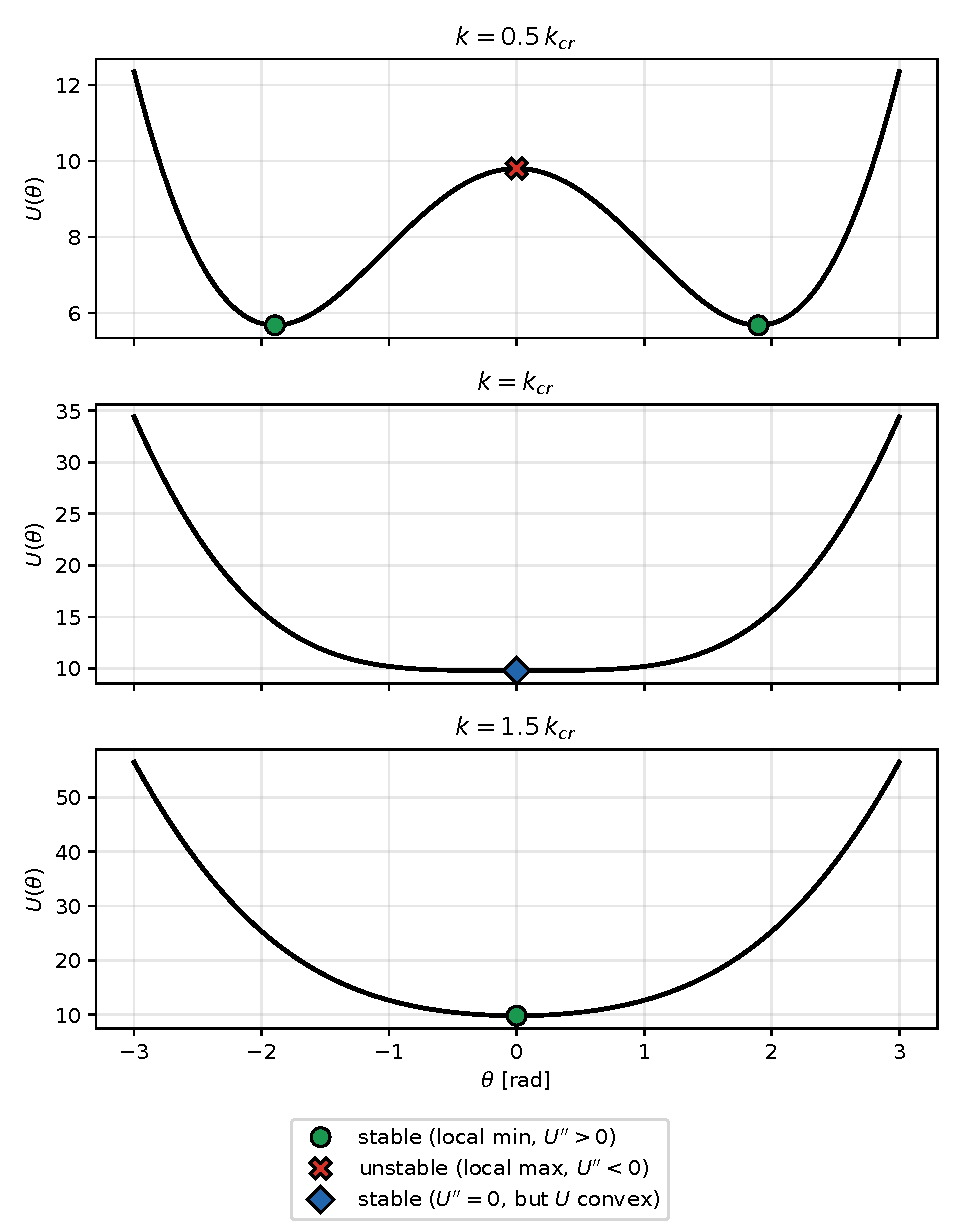
\includegraphics[width=0.72\textwidth]{fig_potential.pdf}
  \caption{$U(\theta)$ for $k=0.5\,\kcr$, $\kcr$, and $1.5\,\kcr$ ($m=\ell=1$, $g=9.8$). Green circles: stable equilibria (local minima). Red X: unstable equilibrium (local maximum). Blue diamond: equilibrium at $k=\kcr$ where $U''(0)=0$; $U$ is convex everywhere in this case, so $\theta=0$ is still a (global) minimum and hence stable --- see Sec.~3(e).}
  \label{fig:U}
\end{figure}

\subsection*{(c) Equilibria}
An equilibrium is a point where the generalized force vanishes, $-\,dU/d\theta = 0$. On the plot this is a \textbf{point of zero slope} of $U(\theta)$. Here
\[
  \frac{dU}{d\theta} = -mg\ell\sin\theta + k\theta = 0
  \quad\Longleftrightarrow\quad
  \theta=0\ \ \text{or}\ \ \frac{\sin\theta}{\theta} = \frac{k}{\kcr}.
\]
\begin{itemize}
  \item $\theta=0$ (upright) is always an equilibrium.
  \item $\sin\theta/\theta$ decreases monotonically from 1 (at $\theta\to0$) to 0 (at $\theta=\pi$), and $|\sin\theta/\theta|\le 1/|\theta|$. So for $k\ge\kcr$ there is no other root, while for $k<\kcr$ there is exactly one pair $\pm\theta^*$ in $(0,\pi)$.
  \item For $k=0.5\,\kcr$: solving $\sin\theta^*/\theta^*=0.5$ numerically gives $\theta^*\approx 1.8955$~rad. (Note $\theta^*>\pi/2$: the mass has swung below the horizontal.)
\end{itemize}
Note that $\theta=\pi$ (hanging straight down) is \emph{not} an equilibrium here, because the torsion spring is wound by $\pi$ there and applies torque $k\pi\neq0$.

\begin{center}
\begin{tabular}{@{}lccc@{}}
\toprule
Case & Equilibria in $[-3,3]$ & $U''(\theta_e)$ & Type \\
\midrule
$k=0.5\,\kcr$ & $0$ & $-4.90$ & unstable (max) \\
              & $\pm1.8955$ & $+8.03$ & stable (min) \\
$k=\kcr$      & $0$ & $0$ & min, but $U''=0$ (see (e)) \\
$k=1.5\,\kcr$ & $0$ & $+4.90$ & stable (min) \\
\bottomrule
\end{tabular}
\end{center}
These are marked in Fig.~\ref{fig:U}.

\subsection*{(d) Stability from $U(\theta)$}
Linearizing about any equilibrium $\theta_e$ with $\theta=\theta_e+\delta$ gives
\[
  m\ell^2\,\ddot\delta + U''(\theta_e)\,\delta = 0 ,
  \qquad U''(\theta) = k - mg\ell\cos\theta ,
\]
the same form as the linearized equation of Sec.~2 with $a = U''(\theta_e)/(m\ell^2)$. So stability corresponds directly to the \textbf{local curvature of $U$} at the equilibrium:
\begin{itemize}
  \item $U''(\theta_e)>0$: $U$ is \textbf{convex} (curves up) around $\theta_e$, like the bottom of a valley: the equilibrium is \textbf{stable}.
  \item $U''(\theta_e)<0$: $U$ is \textbf{concave} (curves down) around $\theta_e$, like the top of a hill: the equilibrium is \textbf{unstable}.
  \item $U''(\theta_e)=0$: the curvature vanishes and this simple test is inconclusive; part (e) resolves this case.
\end{itemize}
The stable frequencies here are $\omega_n=\sqrt{4.9}=2.21$~rad/s at $\theta=0$ for $k=1.5\,\kcr$, and $\sqrt{8.03}=2.83$~rad/s at $\pm\theta^*$ for $k=0.5\,\kcr$. The markers in Fig.~\ref{fig:U} are color-coded accordingly (green = stable, red = unstable, blue = the borderline $k=\kcr$ case, resolved below).

\subsection*{(e) The critical case $k=\kcr$}
Setting $k=mg\ell$, the second derivative of the potential is
\[
  U''(\theta) = k - mg\ell\cos\theta = mg\ell\big(1-\cos\theta\big) \;\ge\; 0 \quad\text{for \emph{every} }\theta,
\]
with equality only at $\theta=0$ (mod $2\pi$). So $U$ is convex everywhere, not just near $\theta=0$: the potential curves upward around every point. By the same curvature criterion as part (d), a potential that curves upward around $\theta=0$ means the upright equilibrium is \textbf{stable} --- this holds even though the curvature happens to vanish exactly at $\theta=0$ itself, since convexity of the whole well around that point is enough to confirm it sits at the bottom. Note that we have proved this analytically above, but making this argument in some form with reference to the plot is enough for full credit.

\paragraph{Why the linearization fails.}
At $k=\kcr$, $a=0$, so the quadratic term in the Taylor expansion of $U$ about $\theta=0$ vanishes:
\[
  U(\theta) = mg\ell\Big(\cos\theta+\tfrac12\theta^2\Big) = mg\ell\Big(1 + \frac{\theta^4}{24} - \cdots\Big).
\]
With the $\theta^2$ term gone, the next term in the expansion --- the quartic term $mg\ell\,\theta^4/24$ --- dominates the local shape of $U$ near $\theta=0$. Its coefficient is positive, so $U$ still curves upward near the origin and the equilibrium is stable, but this is information the quadratic (linearized dynamics) approximation simply cannot see: whenever the linear term vanishes, the next-order term in the Taylor expansion takes over, and reading off stability requires looking at that nonlinear term instead. Equivalently, in the equation of motion, expanding $\sin\theta$ gives $\thdd \approx -\frac{g}{6\ell}\theta^3$ near the origin: a nonlinear, but still restoring, term. (Consequence: oscillation period depends on amplitude, $T\propto 1/A$, unlike a linear oscillator.)

%=====================================================================
\section{Numerical Simulation}

\paragraph{Setup.}
With state $\mathbf x = (\theta,\thd)^T$, the dynamics take the form $\dot{\mathbf x} = f(\mathbf x)$ with
\[
  f(\mathbf x) = \begin{bmatrix}\thd\\[4pt] \dfrac{g}{\ell}\sin\theta - \dfrac{k}{m\ell^2}\theta\end{bmatrix}.
\]
Here are solutions integrated with \texttt{scipy.integrate.solve\_ivp} (RK45, the same Dormand--Prince pair as \texttt{ode45}), using \texttt{rtol}$=10^{-10}$, \texttt{atol}$=10^{-12}$, on $t\in[0,60]$~s. For each $k\in\{0.5,1,1.5\}\kcr$, the same batch of $N=20$ runs was integrated with $\thd(0)=0$ and $\theta(0)\sim U(-3,3)$~rad. (Random seed 2, chosen as the first seed that gave a batch with at least one above-barrier run for the $k=0.5\kcr$ separatrix discussion; only about 7\% of the sampling range produces that.) As a sanity check, energy is conserved to a relative drift below $4\times10^{-9}$ for all runs, so the integration is accurate.

\subsection*{(a)--(b) Phase-plane plots}

\begin{figure}[H]
  \centering
  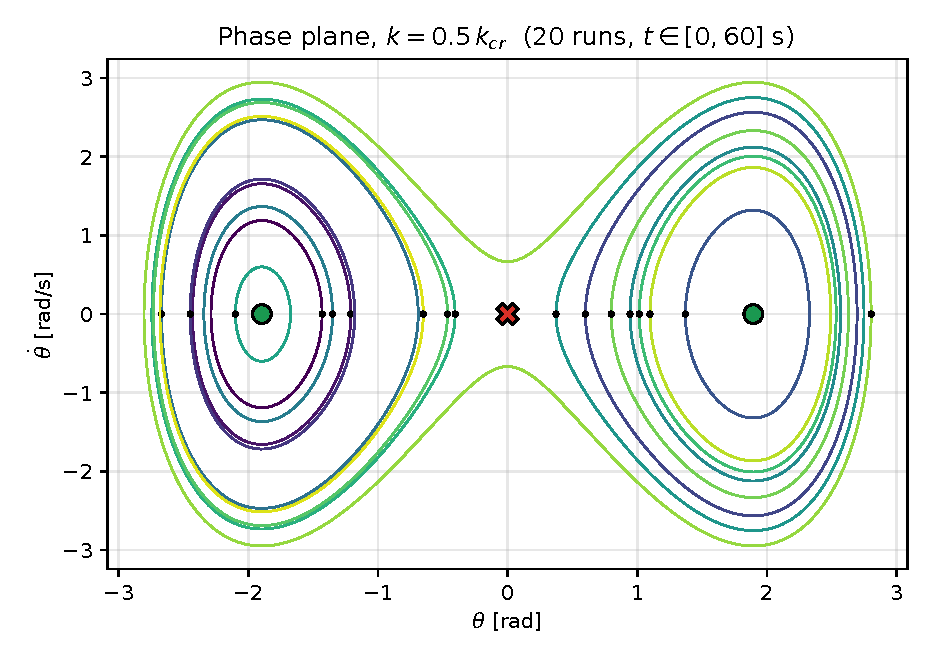
\includegraphics[width=0.66\textwidth]{fig_phase_05.pdf}
  \caption{Phase plane, $k=0.5\,\kcr$. Black dots: initial conditions. Green circles: stable equilibria $\pm\theta^*$; red X: unstable equilibrium at the origin.}
  \label{fig:ph05}
\end{figure}
\begin{figure}[H]
  \centering
  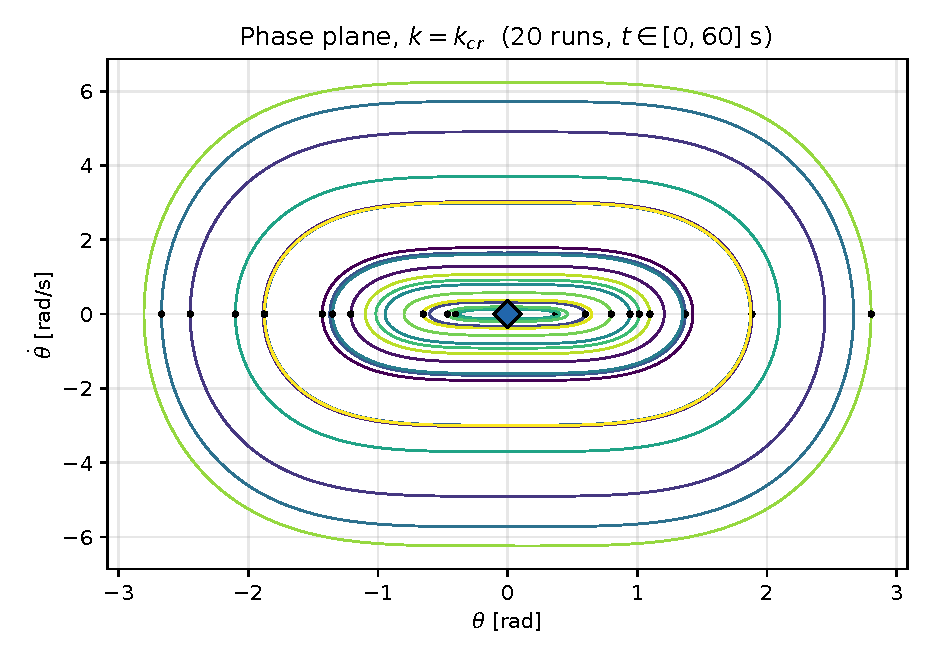
\includegraphics[width=0.66\textwidth]{fig_phase_10.pdf}
  \caption{Phase plane, $k=\kcr$ (blue diamond: the $k=\kcr$ equilibrium, $U''(0)=0$ but stable by convexity --- Sec.~3(e)).}
  \label{fig:ph10}
\end{figure}
\begin{figure}[H]
  \centering
  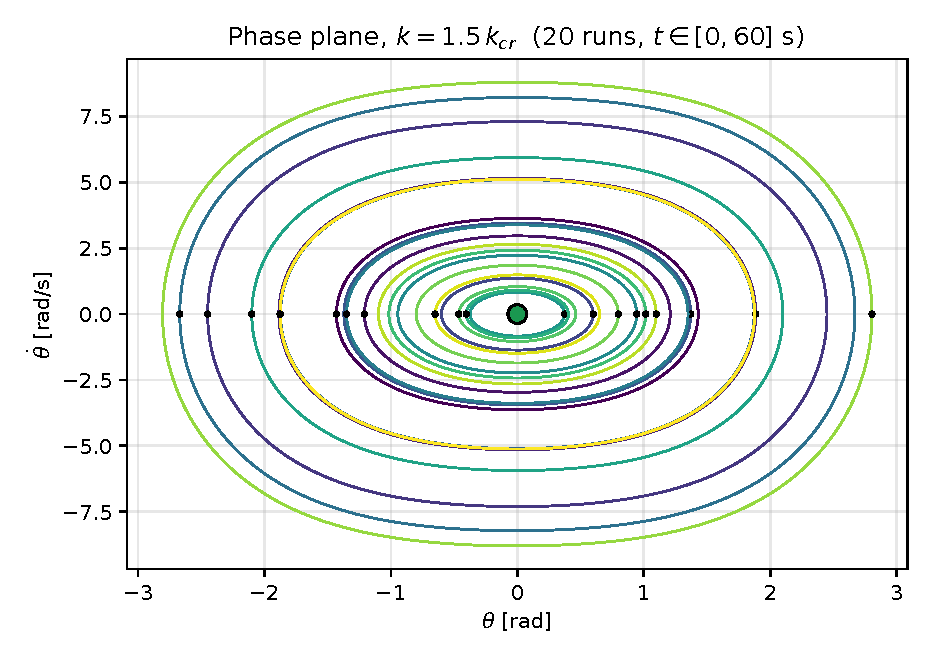
\includegraphics[width=0.66\textwidth]{fig_phase_15.pdf}
  \caption{Phase plane, $k=1.5\,\kcr$.}
  \label{fig:ph15}
\end{figure}

\paragraph{Observations.}
Every trajectory is a closed curve, since each is a level set of the conserved energy $E$. Nothing spirals into or out of an equilibrium because there is no damping.

\begin{itemize}
  \item $k=1.5\,\kcr$ (Fig.~\ref{fig:ph15}): closed loops around the origin, elliptical near the origin with $\dot\theta_{\max}/\theta_{\max}\approx\omega_n=2.21$~s$^{-1}$, becoming more rounded at large amplitude. The origin is a center: stable, as predicted ($a=4.9>0$).
  \item $k=\kcr$ (Fig.~\ref{fig:ph10}): this is the case the linearization could not settle. The orbits are again closed loops around the origin. This confirms the nonlinear stability conclusion of Sec.~3(e), and the equilibrium is \emph{stable but not asymptotically stable}.
  \item $k=0.5\,\kcr$ (Fig.~\ref{fig:ph05}): the origin is a saddle (unstable); runs starting on either side of it are pushed away from it and circulate around one of the two stable equilibria $\pm\theta^*$. One run with $\theta(0)=2.80$ has enough energy to pass over the hump and encloses both wells.
\end{itemize}

\begin{figure}[H]
  \centering
  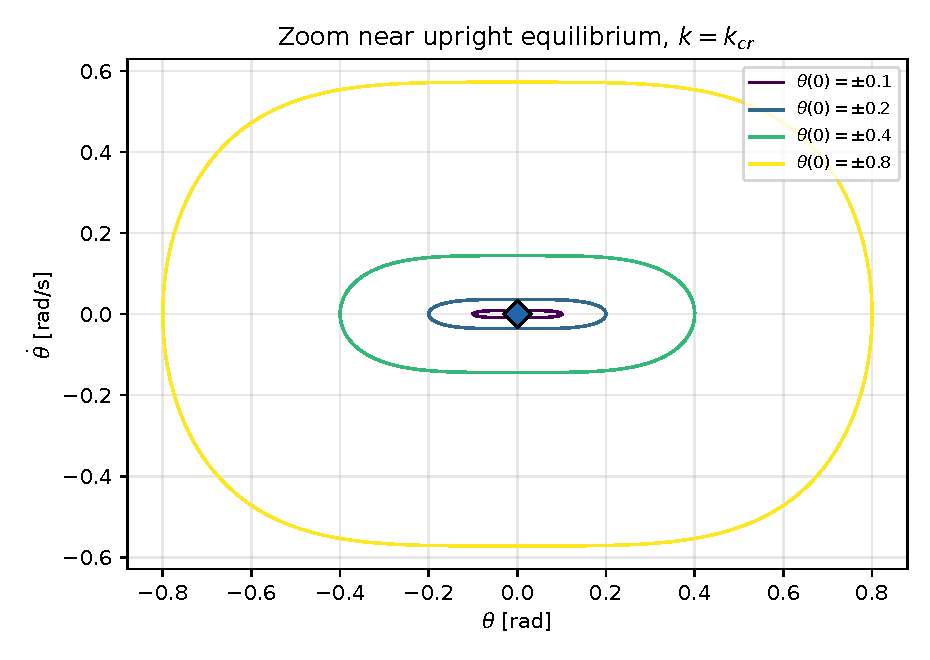
\includegraphics[width=0.66\textwidth]{fig_phase_cr_zoom.pdf}
  \caption{$k=\kcr$: small-amplitude runs ($\theta(0)=\pm0.1,\pm0.2,\pm0.4,\pm0.8$), each integrated for 1.5 estimated periods. The orbits stay arbitrarily close to the origin if started close, confirming the stability predicted in Sec.~3(e) from the convexity of $U$.}
  \label{fig:zoom}
\end{figure}

\subsection*{(c) Separatrix for $k=0.5\,\kcr$}

As the problem statement notes, there is no damping here, so trajectories don't actually converge to $\pm\theta^*$ -- they orbit forever -- and strictly speaking there are no basins of attraction. There is still a well-defined \emph{separatrix}: the curve that divides initial conditions that remain confined to oscillate about $-\theta^*$, about $+\theta^*$, or (if they carry enough energy) swing past both.

\paragraph{Finding it as a trajectory (per the hint).}
Since $E=\tfrac12 m\ell^2\thd^2+U(\theta)$ is conserved, every trajectory is a level curve of $E$, and the separatrix is \emph{itself a trajectory}: the one passing through the saddle (unstable equilibrium) at the origin, with energy
\[
E_{sep} = U(0) = mg\ell = 9.8 .
\]
Generating it numerically requires an initial condition that lies exactly on this level curve. The saddle itself, $(\theta,\thd)=(0,0)$, is a fixed point, so the curve's other zero-velocity point is used instead: since $U$ is even and $U(0)=mg\ell$, the equation $U(\theta_{\max})=U(0)$ has a second root $\theta_{\max}>0$,
\[
mg\ell\cos\theta_{\max} + \tfrac12 k\theta_{\max}^2 = mg\ell
\quad\xrightarrow{\;m=\ell=1,\,k=4.9\;}\quad
\theta_{\max}\approx 2.783~\text{rad.}
\]
Releasing the pendulum from rest at $\theta(0)=\theta_{\max}$, $\thd(0)=0$ puts it exactly on the separatrix (zero velocity $\Rightarrow$ $E_0=U(\theta_{\max})=E_{sep}$). Integrating forward in time traces one half of the right-hand loop; integrating backward in time traces the other half. The trajectory only reaches the saddle asymptotically as $t\to\pm\infty$, so a long but finite integration ($t=\pm400$~s) traces the loop essentially all the way around: the simulated curve passes within $1.2\times10^{-6}$~rad of the saddle, with energy conserved to $2\times10^{-10}$. The left-hand loop can be found by starting at $-\theta_{\max}$ instead of $\theta_{\max}$.


\begin{figure}[H]
  \centering
  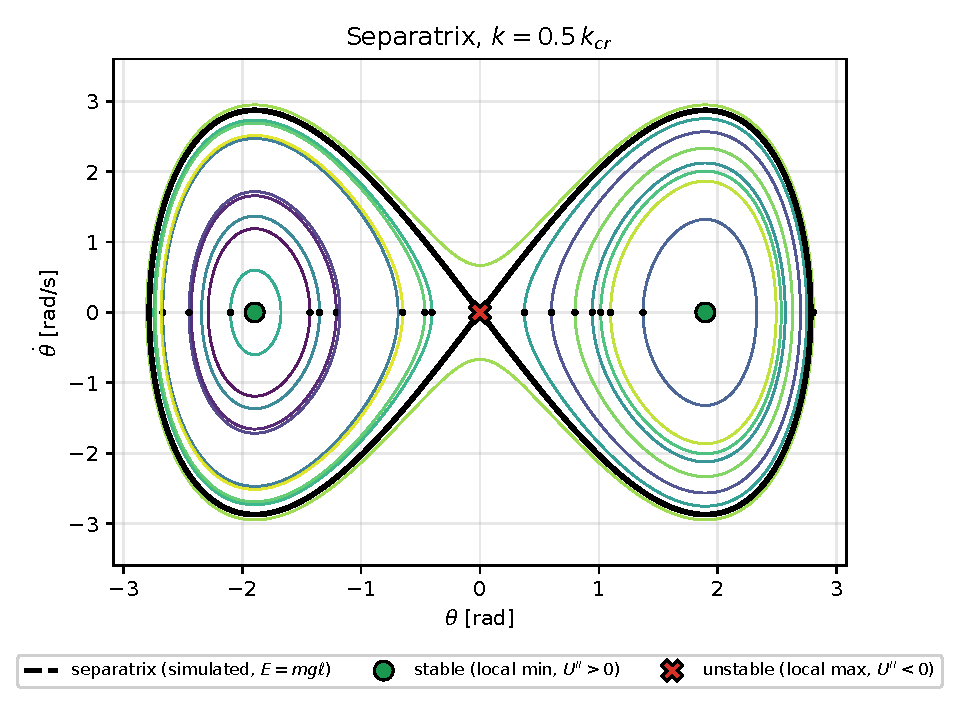
\includegraphics[width=0.72\textwidth]{fig_separatrix.pdf}
  \caption{Phase plane for $k=0.5\,\kcr$ with the separatrix (dashed black), obtained by simulating a trajectory released from rest at $\theta=\theta_{\max}=2.783$. Runs inside the left loop circulate around $-\theta^*$, runs inside the right loop around $+\theta^*$; the one run outside (started at $\theta(0)=2.80$) encloses both loops.}
  \label{fig:sep}
\end{figure}

Because the batch's initial conditions have $\thd(0)=0$, $E_0=U(\theta_0)$, and:
\begin{itemize}
  \item $|\theta_0|<\theta_{\max}$ (with $\theta_0\ne0$): $E_0<E_{sep}$, so the run is confined to oscillate in one well. The sign of $\theta_0$ selects the well. Sample: 11 runs in the left well, 8 in the right well.
  \item $|\theta_0|>\theta_{\max}$: $E_0>E_{sep}$, so the run swings past the hump and orbits both wells. Sample: 1 run (with $\theta_0=2.80$).
\end{itemize}

No trajectories cross the separatrix.

%=====================================================================
\appendix
\section{Code}
The script below generates all figures and numbers quoted above.
\lstinputlisting{pset1_sim.py}

\end{document}
